\section{}
\[
H(s)=\frac{s^2-100}{s+1}=\frac{(s-10)(s+10)}{s+1}\,.
\]
\subsection{Bode-Diagramm}
\begin{center}
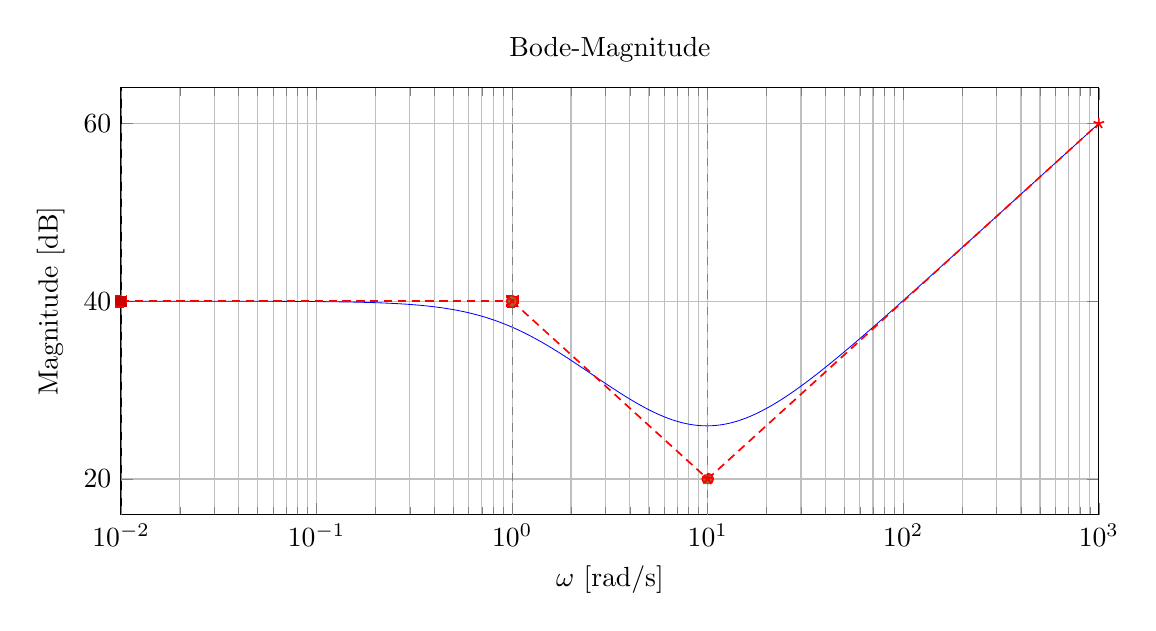
\begin{tikzpicture}
\begin{semilogxaxis}[
  width=14cm,height=7cm,
  xmin=1e-2,xmax=1e3,
  xlabel={$\omega$ [rad/s]},
  ylabel={Magnitude [dB]},
  grid=both,
  ytick distance=20,
  title={Bode-Magnitude}
]
\addplot[
  domain=1e-2:1e3,
  samples=600,
  mark=none,
  line width=0.3pt,
  blue
] {40*ln(sqrt(100 + x^2))/ln(10) - 20*ln(sqrt(1 + x^2))/ln(10)};
\addplot+[domain=1e-2:1,samples=2,dashed,dash pattern=on 3pt off 2pt,line width=0.6pt,red] {40};
\addplot+[domain=1:1e1,samples=2,dashed,dash pattern=on 3pt off 2pt,line width=0.6pt,red] {40 - 20*ln(x)/ln(10)};
\addplot+[domain=1e1:1e3,samples=2,dashed,dash pattern=on 3pt off 2pt,line width=0.6pt,red] {20 + 20*ln(x/10)/ln(10)};
\draw[gray,dashed] (rel axis cs:0,0) -- (rel axis cs:0,1);
\draw[gray,dashed] (axis cs:1,\pgfkeysvalueof{/pgfplots/ymin}) -- (axis cs:1,\pgfkeysvalueof{/pgfplots/ymax});
\draw[gray,dashed] (axis cs:10,\pgfkeysvalueof{/pgfplots/ymin}) -- (axis cs:10,\pgfkeysvalueof{/pgfplots/ymax});
\node[gray,anchor=south east] at (axis cs:1,\pgfkeysvalueof{/pgfplots/ymax}) {\scriptsize Pol $\omega_p=1$};
\node[gray,anchor=south east] at (axis cs:10,\pgfkeysvalueof{/pgfplots/ymax}) {\scriptsize Nullstellen $\omega_z=10$ (LHP \& RHP)};
\end{semilogxaxis}
\end{tikzpicture}
\vspace{6mm}
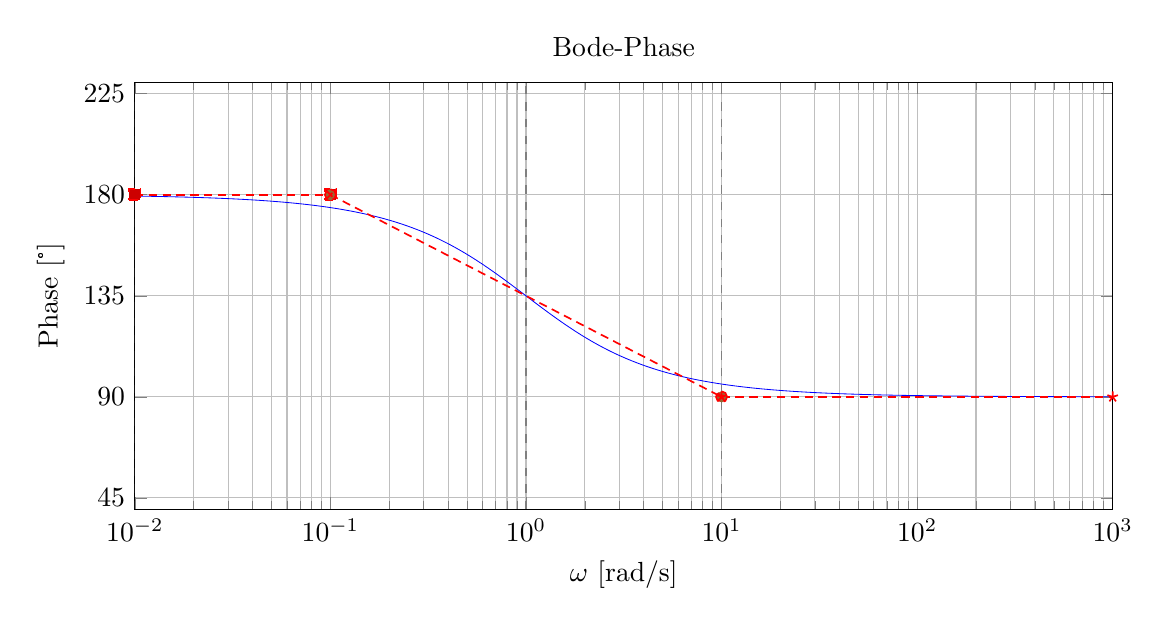
\begin{tikzpicture}
\begin{semilogxaxis}[
  width=14cm,height=7cm,
  xmin=1e-2,xmax=1e3,
  ytick distance=45,
  ymin=40,ymax=230,
  xlabel={$\omega$ [rad/s]},
  ylabel={Phase [°]},
  grid=both,
  title={Bode-Phase}
]
\addplot[
  domain=1e-2:1e3,
  samples=600,
  mark=none,
  line width=0.3pt,
  blue
] {180 - atan(x)};
\addplot+[domain=1e-2:1e-1,samples=2,dashed,dash pattern=on 3pt off 2pt,line width=0.6pt,red] {180};
\addplot+[domain=1e-1:1e1,samples=2,dashed,dash pattern=on 3pt off 2pt,line width=0.6pt,red] {135 - 45*ln(x)/ln(10)};
\addplot+[domain=1e1:1e3,samples=2,dashed,dash pattern=on 3pt off 2pt,line width=0.6pt,red] {90};
\draw[gray,dashed] (rel axis cs:0,0) -- (rel axis cs:0,1);
\draw[gray,dashed] (axis cs:1,\pgfkeysvalueof{/pgfplots/ymin}) -- (axis cs:1,\pgfkeysvalueof{/pgfplots/ymax});
\draw[gray,dashed] (axis cs:10,\pgfkeysvalueof{/pgfplots/ymin}) -- (axis cs:10,\pgfkeysvalueof{/pgfplots/ymax});
\node[gray,anchor=south east] at (axis cs:1,\pgfkeysvalueof{/pgfplots/ymax}) {\scriptsize Pol $\omega_p=1$};
\node[gray,anchor=south east] at (axis cs:10,\pgfkeysvalueof{/pgfplots/ymax}) {\scriptsize Nullstellen $\omega_z=10$ (LHP \& RHP)};
\end{semilogxaxis}
\end{tikzpicture}
\end{center}
\newpage

\subsection{Erklärung}
\begin{description}[leftmargin=1.2em,labelsep=.6em,font=\bfseries]

\item[1. Normalform herstellen.]
\[
H(s)=\frac{(s-10)(s+10)}{s+1}
=-100\,(1-sT_{z1})\,(1+sT_{z2})\cdot\frac{1}{1+sT_p}
\]
mit
\[
K_0=-100,\quad r=0,\quad T_{z1}=\tfrac{1}{10},\quad T_{z2}=\tfrac{1}{10},\quad T_p=1.
\]
\[
\underline{F}_1(s)=\bigl(1-sT_{z1}\bigr)\ \text{(RHP-Nullstelle)},\]
\[\underline{F}_2(s)=\bigl(1+sT_{z2}\bigr)\ \text{(LHP-Nullstelle)},\]
\[\underline{F}_3(s)=\tfrac{1}{1+sT_p}\ \text{(Pol)}.\]

\item[2. Eckfrequenzen bestimmen und sortieren.]
\[
\omega_{p}=1\,\mathrm{rad/s},\qquad
\omega_{z1}=\omega_{z2}=10\,\mathrm{rad/s},\qquad
\omega_p<\omega_z.
\]

\item[3. Startpunkt des Amplitudengangs festlegen (Geradennäherung).]
Setze \(\omega_{\min}=\omega_p=1\).
\[
F_{\mathrm{dB}}(\omega_{\min})=20\log_{10}\!\big(|K_0\underline{F}_{ges}^*(0)|\,\omega_{\min}^{\,r}\big)=20\log_{10}100=40\,\mathrm{dB}.
\]
Ankerpunkt: \(40\,\mathrm{dB}\) bei \(\omega=1\).

\item[4. Verlauf links vom Startpunkt zeichnen.]
Für \(\omega<1\) horizontale Asymptote bei \(40\,\mathrm{dB}\) (Anfangssteigung \(r\cdot 20\,\mathrm{dB/dec}=0\)). Waagrechte Gerade links von der kleinsten Eckfrequenz eintragen.

\item[5. Steigungswechsel an den Eckfrequenzen eintragen.]
Ab \(\omega=1\): Pol \(\Rightarrow\) Steigungswechsel \(-20\,\mathrm{dB/dec}\).
Ab \(\omega=10\): zwei Nullstellen \(\Rightarrow\) zusätzl. \(+40\,\mathrm{dB/dec}\).
Netto:
\[
\begin{cases}
40\,\mathrm{dB},& \omega<1,\\
40-20\log_{10}\omega,& 1\le\omega<10,\\
20+20\log_{10}(\omega/10),& \omega\ge 10.
\end{cases}
\]

\item[6. Eckabrundungen korrekt berücksichtigen.]
Einfacher Pol bei \(\omega=1\): \(-3\,\mathrm{dB}\) am Knick \(\Rightarrow |H(j1)|_{\mathrm{dB}}\approx 40-3=37\,\mathrm{dB}\).
Zwei Nullstellen bei \(\omega=10\): \(+6\,\mathrm{dB}\) am Knick \(\Rightarrow |H(j10)|_{\mathrm{dB}}\approx 20+6=26\,\mathrm{dB}\).

\item[7. Phasenstartwert festlegen.]
Verwende die Regel für $K_0\underline{F}_{ges}^*(0) <0$:
\[
\varphi(0)=-180^\circ + r\cdot 90^\circ= -180^\circ
\]
(Darstellung im Plot um \(+360^\circ\) verschoben \(\Rightarrow\) Start bei \(+180^\circ\)).

\item[8. Phasenänderung durch Pol und Nullstellen eintragen.]
Pol bei \(\omega_p\) bewirkt eine Phasenänderung \(-90^\circ\) über \([0.1,10]\).
Nullstellen bei \(\omega_z\): LHP-Nullstelle \(+90^\circ\) und RHP-Nullstelle \(-90^\circ\), beide über \([1,100]\). die \(+90^\circ\) und \(-90^\circ\) der beiden Nullstellen kompensieren sich zu \(0^\circ\). Netto wirkt in $[1,10]$ nur der Pol.
Näherung (mit Phasenverschiebung um \(+360^\circ\) gezeigt):
\[
\varphi(\omega)\approx
\begin{cases}
180^\circ,& \omega\le 0.1,\\
135^\circ-45^\circ\log_{10}\omega,& 0.1<\omega<10,\\
90^\circ,& \omega\ge 10.
\end{cases}
\]

\item[9. Grenzwerte und Konsistenz prüfen.]
DC: \(|H(0)|=100\Rightarrow 40\,\mathrm{dB}\); \(\varphi(0)=-180^\circ\) (gezeigt als \(+180^\circ\)).
HF: \(|H(j\omega)|\sim \omega^2/\omega= \omega \Rightarrow 20\log_{10}\omega + 20\,\mathrm{dB}\).

\end{description}

\subsubsection*{Stückweise Näherungen (für die Skizze)}
\[
|H(j\omega)|_{\mathrm{dB}}\approx
\begin{cases}
40,& \omega\ll 1,\\[2pt]
40-3,& \omega=1,\\[2pt]
40-20\log_{10}\omega,& 1\ll\omega\ll 10,\\[2pt]
20+6,& \omega=10,\\[2pt]
20+20\log_{10}(\omega/10),& \omega\gg 10,
\end{cases}
\]
\[
\varphi(\omega)\ (\text{Darstellung }+360^\circ)\approx
\begin{cases}
180^\circ,& \omega\le 0.1,\\[2pt]
135^\circ-45^\circ\log_{10}\omega,& 0.1<\omega<10,\\[2pt]
90^\circ,& \omega\ge 10.
\end{cases}
\]

\newpage